% This must be in the first 5 lines to tell arXiv to use pdfLaTeX, which is strongly recommended.
\pdfoutput=1

\documentclass[11pt]{article}

\usepackage[preprint]{acl}

\usepackage{times}
\usepackage{latexsym}
\usepackage[T1]{fontenc}
\usepackage[utf8]{inputenc}
\usepackage{microtype}
\usepackage{inconsolata}
\usepackage{mathtools}

%%%% My packages
\usepackage{svg}
\usepackage{textcomp}  % Required for encoding \textbigcircle
\usepackage{scalerel}  % Required for emoji \scalerel
\usepackage{lipsum}
\usepackage{tikz}
\usetikzlibrary{fit,arrows,quotes,calc,automata,positioning,backgrounds,arrows.meta,bending,shapes,snakes,matrix,shadows,fadings,decorations,decorations.text,decorations.markings,shapes.geometric,shadings}
\usepackage{subcaption}
\usepackage{amsmath}
\usepackage{amsfonts}
\usepackage{amssymb}
\usepackage[english]{babel}
\usepackage{mathtools}
\usepackage{hyperref}
\usepackage{mdframed}
\usepackage{csvsimple}
\usepackage{subcaption}
\usepackage{multirow}
\usepackage{tcolorbox}
\usepackage{siunitx}
\sisetup{
  round-mode=uncertainty,
  % round to 3 significant figures
  round-precision=2,
  scientific-notation = false,
  % drop trailing zeros
  round-pad=false,
  add-integer-zero=false,
  add-decimal-zero=false,
  output-decimal-marker={.},
  group-digits=integer,
  group-separator={,},
  separate-uncertainty = true,
  detect-all,
  detect-weight=true,
  detect-inline-weight=math,
}
\usepackage{amssymb}% http://ctan.org/pkg/amssymb

\definecolor{myRED}{HTML}{D50000}
\definecolor{myBLUE}{HTML}{00FBFF}
\definecolor{myDARKBLUE}{HTML}{007ACC}
\definecolor{myGREEN}{HTML}{00FF00}
\definecolor{myMAGENTA}{HTML}{C200D6}

\def\strong#1{\textbf{#1}}

% Custom command for metrics
\newcommand{\metric}[1]{\texttt{#1}}
\usepackage{soul}
\setul{0.5ex}{0.2ex}
\newcommand{\ulcolor}[2][myRED]{\setulcolor{#1}\ul{#2}}

\title{Prompt Length Optimization with Reinforcement Learning}

\author{Aldan Creo \and Atharv Nair \\
  University of California, San Diego \\
  \texttt{acreo@ucsd.edu}, \texttt{a6nair@ucsd.edu}}

\begin{document}
\maketitle
\begin{abstract}
  % Idea: we frame prompt discovery as an RL problem to find minimal prompts that maximize posterior probability
  Abstract here
\end{abstract}

\section{Introduction}
\label{sec:introduction}

% Idea: we're doing prompt optimization for LMs, this has applications in e.g. security research (find jailbreaks) or improving performance (e.g. improving prompts to maximize their effectiveness on downstream tasks)
Language models (LMs) have grown in popularity due to their applicability on a range of NLP tasks. Prompt optimization is an area of research that aims to find a set of tokens that is likely to elicit a specific response from the model, 

% Idea: highlight gap between likelihood-only search and static pruning
Many prompt search methods chase likelihood and ignore length. Pruning approaches drop tokens but do not adapt during optimization. We want both goals at once: keep the prompt likely under the model and cut tokens when we can.

% Idea: explain our external policy and scope (plug-in optimizer, no retrieval/safety)
We train a small external policy instead of a new language model. The policy decides when to shrink, keep, or grow a prompt, while any plug-in optimizer adjusts tokens. We do not design a new optimizer and accept the limits of whichever one is used. We also avoid retrieval and safety objectives; we only balance likelihood and length.

\begin{figure*}[t]
  \centering
  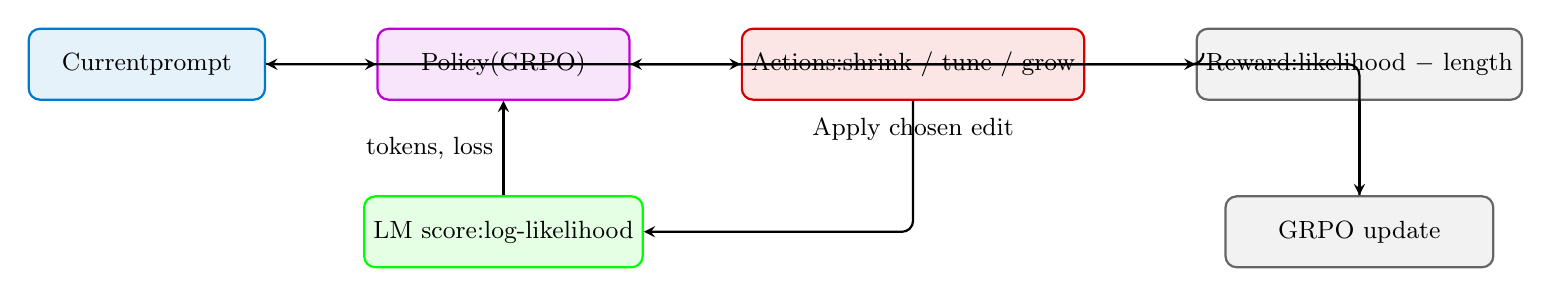
\begin{tikzpicture}[>=stealth, node distance=1.2cm and 1.4cm, rounded corners, font=\small]
    % Nodes
    \node[draw=myDARKBLUE, fill=myDARKBLUE!10, thick, align=center, minimum width=3cm, minimum height=0.9cm] (prompt) {Current\newline prompt};
    \node[draw=myMAGENTA, fill=myMAGENTA!10, thick, align=center, minimum width=3.2cm, minimum height=0.9cm, right=of prompt] (policy) {Policy\newline (GRPO)};
    \node[draw=myRED, fill=myRED!10, thick, align=center, minimum width=3.4cm, minimum height=0.9cm, right=of policy] (actions) {Actions:\newline shrink / tune / grow};
    \node[draw=myGREEN, fill=myGREEN!10, thick, align=center, minimum width=3.4cm, minimum height=0.9cm, below=of policy] (lm) {LM score:\newline log-likelihood};
    \node[draw=black!60, fill=black!5, thick, align=center, minimum width=3.4cm, minimum height=0.9cm, right=of actions] (reward) {Reward:\newline likelihood $-$ length};
    \node[draw=black!60, fill=black!5, thick, align=center, minimum width=3.4cm, minimum height=0.9cm, below=of reward] (update) {GRPO update};

    % Arrows
    \draw[->, thick] (prompt) -- (policy);
    \draw[->, thick] (policy) -- (actions);
    \draw[->, thick] (actions) |- (lm);
    \draw[->, thick] (lm) -- node[left]{tokens, loss} (policy);
    \draw[->, thick] (actions) -- (reward);
    \draw[->, thick] (reward) -- (update);
    \draw[->, thick] (update) |- (policy);
    \draw[->, thick] (actions.east) ++(0.6,0) -- ++(0.9,0) |- (prompt.east);
    \node[align=center, below=0.1cm of actions] (loopnote) {Apply chosen edit};
  \end{tikzpicture}
  \caption{Policy loop: given a prompt, we choose one of three edits (shrink, tune, grow), score the new prompt with the LM, and update the policy with a reward that balances likelihood and length.}
  \label{fig:method}
\end{figure*}

\section{Related Work}
\label{sec:related}

% Idea: prompt optimization is popular, many methods exist
Prompt optimization is a very active area of research, with many authors proposing a variety of techniques. Therefore, we group prior work into four areas:

% Idea: gradient-based discrete prompt optimization
\paragraph{Discrete optimization.} These methods keep prompts in the token space and use gradients to move among words. HotFlip-style edits and \citet{shin2020autoprompt} pick candidate tokens with gradient signals. \citet{wen2023hard} smooth the search with continuous helpers and then project back to tokens. Adversarial suffix work like \citet{zou2023universal} and faster probe sampling \citep{zhao2024accelerating} show that gradient-guided discrete search can find strong suffixes when we have white-box access.

% Idea: continuous prompt optimization and projection
\paragraph{Continuous optimization.} Soft prompt tuning swaps hard tokens for learned embedding vectors that we train with backpropagation \citep{lester2021power}. Later work looks at safety and robustness in the embedding space \citep{schwinn2024soft}. More recently, \citet{wang2025dpro} study direct prompt optimization with continuous representations, using stronger goals to narrow the gap between soft prompts and discrete use.

% Idea: prompt compression for efficiency
\paragraph{Prompt compression.} To cut inference cost, coarse-to-fine pruning methods compress demonstrations and questions with perplexity signals from a smaller LM, as in LLMLingua \citep{jiang2023llmlingua} and its distilled follow-up \citep{pan2024llmlingua2}. Gist tokens \citep{mu2023gist} learn short continuous summaries; context-aware compression uses sentence encodings \citep{liskavets2024prompt}. TACO-RL \citep{shandilya2024taco} adds task-aware rewards to compression to keep outputs accurate under fixed length budgets.

% Idea: reinforcement learning for prompt editing and safety
\paragraph{Reinforcement learning.} RL has been used to optimize prompts or policies that pick edits over sequences \citep{ramamurthy2022rlnlp}, and to align or adversarially steer LMs with discrete action spaces. Our work links to this line by viewing length control as a policy that decides when to compress versus improve likelihood, not only by tuning embeddings.

\section{Problem Formulation}
\label{sec:problem}

% Idea: define the goal, objective, and constraints
We are given a fixed prefix $x_{\text{pref}}$, a target completion $y$, and a trainable suffix $s$ of up to $L_{\max}$ tokens. We do not change model weights; we only edit $s$. At each step we pick an action that changes $|s|$ or refines its tokens, and we score the resulting prompt with the log-likelihood of $y$ under the frozen language model.

We cast this as a finite-horizon Markov decision process (MDP). A state $z$ stores the current suffix length $|s|$, the current log-likelihood $\ell = \log p_\theta(y\mid x_{\text{pref}}, s)$, a length-normalized likelihood $\ell/\ell_0$, and the fraction of episode steps used. Actions are $a\in\{\text{optimize},\text{shrink},\text{grow}\}$ and only affect the suffix.

The reward trades off likelihood and length. At the end of each episode we compute
\begin{equation}
  r = \alpha \cdot \tilde \ell\; -\; \beta \cdot \frac{|s|}{L_{\max}},
\end{equation}
where $\tilde \ell$ is a per-token log-likelihood normalized within the batch, $\alpha>0$ weighs accuracy, and $\beta>0$ penalizes length. Intermediate steps receive discounted copies of this terminal reward so that all actions that led to the final suffix share credit. Episodes last a fixed number of steps; prefix and completion tokens never change.

\subsection{State Space}
\label{subsec:state}

% Idea: simple five-dimensional state
We use a five-dimensional state vector per rollout: (1) normalized length $|s|/|s_0|$; (2) current length $|s|$; (3) current log-likelihood $\ell$; (4) likelihood ratio $\ell/(\ell_0+\varepsilon)$; and (5) progress in the episode $t/T$. These features are cheap to compute and keep the policy lightweight.

\subsection{Action Space}
\label{subsec:actions}

% Idea: three discrete actions that only touch the suffix
We allow three actions: \emph{optimize} (run the inner optimizer on the current suffix), \emph{shrink} (drop one active suffix token), and \emph{grow} (add one active suffix token up to $L_{\max}$). Prefix and completion stay fixed.

\subsection{Reward Function}
\label{subsec:reward}

% Idea: terminal reward with likelihood--length trade-off
The reward in \S\ref{sec:problem} combines normalized per-token log-likelihood with a linear length penalty. We discount it back over episode steps with factor $\gamma$ so earlier actions share credit. We do not add extra terms for safety or retrieval.

\section{Method}
\label{sec:method}

% Idea: describe pipeline from inputs to policy and inner optimizers
We pair a frozen language model with a small policy network. The policy decides when to shrink, grow, or call an inner optimizer; the inner optimizer improves the suffix tokens or embeddings. We train the policy with Group Relative Policy Optimization (GRPO) while leaving the language model untouched.

\subsection{Policy Network Architecture}
\label{subsec:policy}

% Idea: lightweight MLP with epsilon-greedy sampling
The policy is a two-layer MLP that maps the five state features to three action logits. We apply a temperature, softmax, and epsilon-greedy mixing to sample actions. We include an entropy bonus and clip ratios as in GRPO to keep updates stable. Exploration rate $\epsilon$ decays each episode; gradients only update the policy parameters.

\subsection{Optimization Modes}
\label{subsec:modes}

% Idea: plug-in inner optimizers for different search spaces
We support three plug-in inner optimizers; the policy is agnostic to which one is used.

\subsubsection{Continuous Optimization}
\label{subsubsec:continuous}

% Idea: optimize suffix embeddings directly
In continuous mode we treat suffix embeddings as learnable parameters, run Adam to maximize log-likelihood, and later project to the nearest tokens for reporting.

\subsubsection{Continuous with Projection}
\label{subsubsec:continuous_proj}

% Idea: add distance regularization to stay near the embedding table
Continuous\_proj adds a distance regularizer that pulls suffix embeddings toward the nearest token embeddings using a chosen metric; at evaluation we project to tokens to score.

\subsubsection{Discrete Optimization}
\label{subsubsec:discrete}

% Idea: gradient-guided token search (GCG)
In discrete mode we run a Greedy Coordinate Gradient (GCG) search over tokens: rank candidate replacements by gradients, test top-$k$ candidates in batches, and keep the best. Length changes are handled by the policy actions.

\subsection{Training Procedure}
\label{subsec:training}

% Idea: batched episodes with per-prompt baselines
We sample multiple rollouts per prompt, run fixed-length episodes, and record states, actions, and log-probs. After an episode we compute the terminal reward, discount it backward, and center advantages per prompt (GRPO) to reduce variance. We then run several GRPO epochs over the stored trajectories with ratio clipping and entropy bonus.

\subsection{Implementation Details}
\label{subsec:implementation}

% Idea: batching, immutable prefix/completion, suffix-only edits
We build batched inputs with immutable prefix and completion tokens and a trainable suffix of fixed maximum length. ModelBatchedInput handles tokenization, attention masks, and embedding assembly for all modes. The agent uses a frozen Pythia-70m model for likelihoods and supports CPU, CUDA, or MPS devices. All edits and gradients stay in the suffix; prefixes and completions are untouched.

\section{Experiments}
\label{sec:experiments}

% Idea: we evaluate on two datasets: ToxicChat and AdvBench

\subsection{Experimental Setup}
\label{subsec:setup}

% Idea: model architecture (Pythia-70m), hyperparameters, datasets

\subsection{Baselines}
\label{subsec:baselines}

% Idea: compare continuous, continuous_proj, and discrete modes
% Idea: compare to naive baselines (no optimization, random)

\subsection{Evaluation Metrics}
\label{subsec:metrics}

% Idea: mean reward, prompt length, likelihood preservation

\subsection{Results}
\label{subsec:results}

% Idea: quantitative results showing trade-offs
% Idea: qualitative examples of discovered prompts

\subsection{Ablation Studies}
\label{subsec:ablation}

% Idea: impact of alpha and beta on compression vs. likelihood
% Idea: impact of GRPO parameters (clip, entropy coefficient)
% Idea: impact of policy network architecture

\section{Discussion}
\label{sec:discussion}

% Idea: RL successfully learns to balance compression and likelihood
% Idea: different modes have different trade-offs
% Idea: limitations and challenges

\section{Conclusion}
\label{sec:conclusion}

% Idea: we demonstrated RL-based prompt length optimization
% Idea: future work: larger models, different tasks, transfer learning

\bibliography{bibliography}

\appendix

\section{Hyperparameters}
\label{app:hyperparameters}

% Idea: complete list of hyperparameters used in experiments

We present the complete set of hyperparameters used in our experiments. All experiments use the Pythia-70m model~\cite{biderman2023pythia} with seed 2262 for reproducibility.

\subsection{Dataset Parameters}

\begin{itemize}
  \item \textbf{Training prompts}: 256
  \item \textbf{Minimum prompt length}: 30 characters
  \item \textbf{Maximum prompt length}: 150 characters
  \item \textbf{Dataset split}: 70\% train, 15\% validation, 15\% test
\end{itemize}

\subsection{Training Parameters}

\begin{itemize}
  \item \textbf{Episodes per prompt}: 3
  \item \textbf{Steps per episode}: 50
  \item \textbf{Initial suffix length}: 16 tokens
  \item \textbf{Maximum suffix length}: 32 tokens
  \item \textbf{Batch size}: 16 prompts
  \item \textbf{Rollouts per prompt}: 4
\end{itemize}

\subsection{Optimization Parameters}

\begin{itemize}
  \item \textbf{Learning rate (embeddings)}: $\alpha_{\text{emb}} = 0.01$
  \item \textbf{Learning rate (policy)}: $\alpha_{\text{policy}} = 0.001$
  \item \textbf{Epsilon (initial)}: $\epsilon_0 = 0.3$
  \item \textbf{Epsilon decay}: $\gamma_{\epsilon} = 0.97$
  \item \textbf{Epsilon (minimum)}: $\epsilon_{\min} = 0.05$
  \item \textbf{Temperature}: $\tau = 1.5$
\end{itemize}

\subsection{Reward Function Parameters}

\begin{itemize}
  \item \textbf{Likelihood weight}: $\alpha = 0.5$
  \item \textbf{Length penalty}: $\beta = -1.5$ (logarithmic)
  \item \textbf{Projection weight}: $w_{\text{proj}} = 0.5$ (continuous\_proj mode)
  \item \textbf{Distance metric}: L2 distance
\end{itemize}

\subsection{GRPO Parameters}

\begin{itemize}
  \item \textbf{GRPO epochs}: 4
  \item \textbf{Clip parameter}: $\epsilon_{\text{clip}} = 0.2$
  \item \textbf{Discount factor}: $\gamma = 0.99$
  \item \textbf{Entropy coefficient}: $\beta_{\text{entropy}} = 0.003$
  \item \textbf{Maximum gradient norm}: 0.5
\end{itemize}

\subsection{Policy Network Architecture}

\begin{itemize}
  \item \textbf{Input dimension}: 5 (state features)
  \item \textbf{Hidden layer size}: 128
  \item \textbf{Output dimension}: 3 (actions)
  \item \textbf{Activation}: ReLU
  \item \textbf{Optimizer}: Adam
\end{itemize}

\subsection{GCG Parameters (Discrete Mode)}

\begin{itemize}
  \item \textbf{GCG steps}: 3
  \item \textbf{Top-k tokens}: 16
  \item \textbf{Candidate batch size}: 32
  \item \textbf{Maximum batch size}: 128
\end{itemize}

\subsection{Evaluation Parameters}

\begin{itemize}
  \item \textbf{Test prompts}: 200
  \item \textbf{Maximum policy steps}: 25
  \item \textbf{Optimization steps}: 5
\end{itemize}

\section{Code Availability}
\label{app:code}

% Idea: provide access to implementation for reproducibility
The complete implementation of our method, including all experiments and evaluation scripts, is publicly available at \url{https://github.com/ACMCMC/prompt-length-optimization}.

\end{document}
